\chapter{Valores e cronograma}
Antes de iniciarmos o projeto buscamos fazer o orçamento
total necessário para sua conclusão e, criamos um cronograma
a ser seguido, para assim termos prazos de conclusão que incentivem
ainda mais o desenvolvimento do trabalho.

\section{Orçamento}
A tabela ~\ref{tab:precos} é uma relação de todos os componentes utilizados e os preços
encontrados no mercado. Os produtos foram procurados na internet em sites como 
AliExpress e Mercado Livre, sempre levando em conta eficiência e custo, para que o
produto final tenha o maior custo-benefício.

\FloatBarrier
\begin{table}[!htbp]
	\centering
	\caption{Orçamento}
	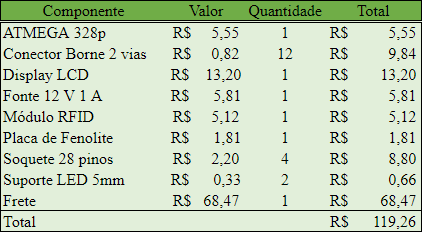
\includegraphics[scale=.75]{imagens/precos}
	\\ \vspace{0.2cm}
	\textbf{Fonte:} Elaborada pelos autores
	\label{tab:precos}
\end{table}
\FloatBarrier

\section{Cronograma}
A tabela ~\ref{tab:cronograma} indica o planejamento do projeto em semanas, o que é esperado que
seja feito e o tempo levado por cada etapa do processo.

\FloatBarrier
\begin{table}[!htbp]
	\centering
	\caption{Cronograma}
	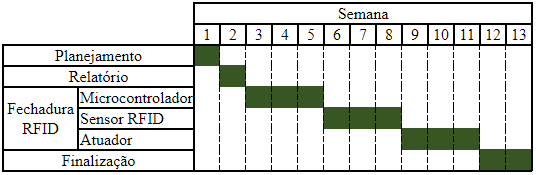
\includegraphics[scale=.75]{imagens/cronograma}
	\\ \vspace{0.2cm}
	\textbf{Fonte:} Elaborada pelos autores
	\label{tab:cronograma}
\end{table}
\FloatBarrier